\begin{frame}{Cinematica}
\begin{columns}
\begin{column}{0.5\textwidth}
\begin{itemize}
    \item<1-> \textcolor{yellow}{rigid link}
    \item<2-> \textcolor{yellow}{piecewise constant curvature}
    \item<3-> piecewise variable curvature
\end{itemize}
\end{column}
\begin{column}{0.8\textwidth}
\only<1>{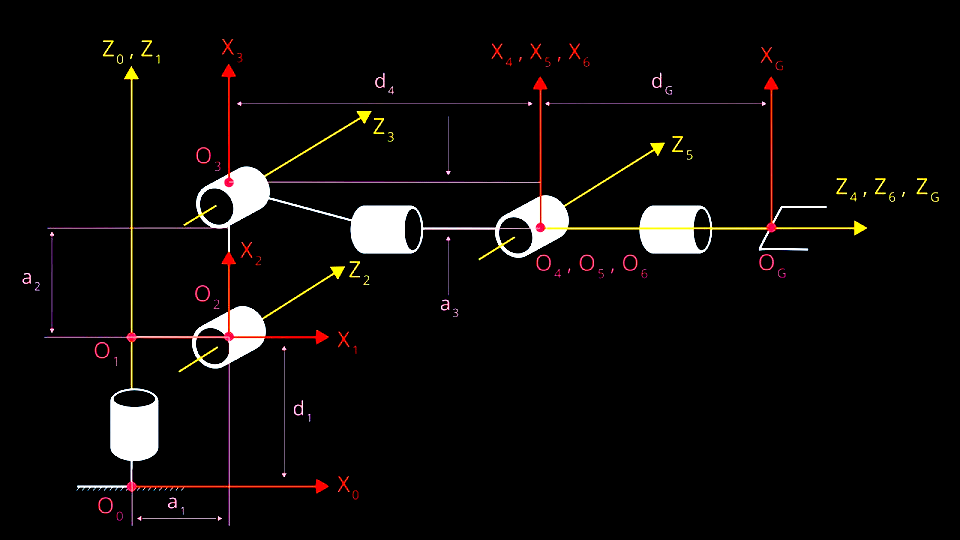
\includegraphics[height=0.7\textheight, trim={0 0 2cm 0},clip]{slide_studio/img_cinematica/kinematics_dh.png}}
\only<2>{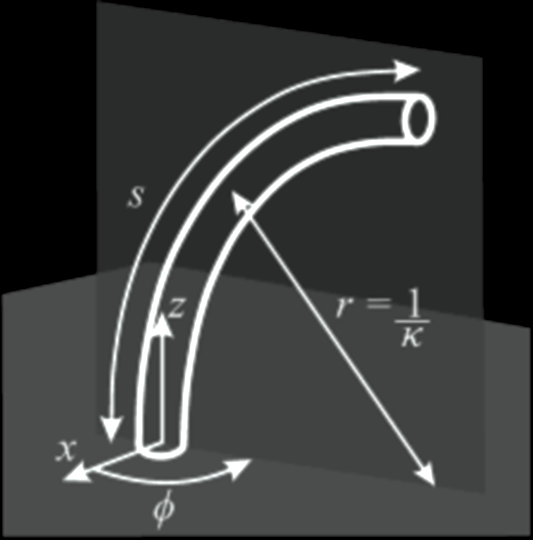
\includegraphics[height=0.7\textheight]{slide_studio/img_cinematica/kinematics_constant_curvature.png}}
\only<3>{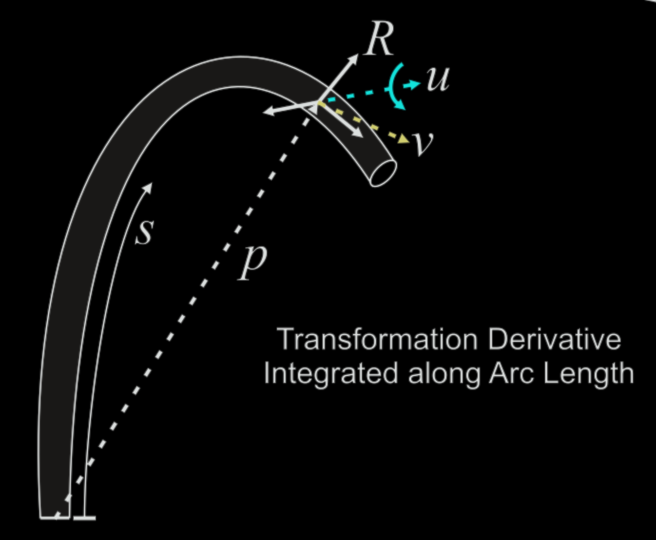
\includegraphics[height=0.7\textheight]{slide_studio/img_cinematica/kinematics_variable_curvature.png}}
\end{column}
\end{columns}
\only<1>{\Reference{Inverse Kinematics on Kuka Arm using ROS and Python}{\url{https://nitishpuri.github.io/posts/robotics/inverse-kinematics-on-kuka-arm-using-ros-and-python/}}{2019}}
\only<2>{\Reference{Design and Kinematic Modeling of Constant Curvature Continuum Robots: A Review}{Webster, Jones}{2010}}
\only<3>{\Reference{A variable curvature continuum kinematics for kinematic control of the bionic handling assistant}{Mahl et al.}{2014}}

\note{
Modello a link rigidi $\to$ link e giunti rotatori e prismatici. Posizione end-effector è funzione dei valori (di angolo, di distanza) del giunto. 

Modello piecewise constant curvature $\to$ segmenti o pezzi, ogni pezzo ha curvatura costante su tutta la lunghezza dell'arco. Posizione è funzione di rotazione e curvatura del segmento. 

Modello piecewise variable curvature $\to$ rimuovo vincolo curvatura costante per tutto il segmento. 
}
\end{frame}